% !TEX root = ./physics_of_fluids.tex
% !TEX TS-program = xelatex
% !TEX encoding = UTF-8 Unicode
\chapter{Boundary conditions and interfaces}
\label{chap:boundary_conditions}
We have seen in the previous chapter how to express mass and momentum conservation at the fluid particle level, and we have derived the corresponding equations for fluid motion. These equations are naturally associated with \textbf{boundary conditions} that either express conservation laws (e.g. no mass flux at a boundary) or peculiar physical processes occurring at a surface (temperature or velocity continuity). In both cases these boundary conditions will be pivoting in the determination of the solution.
\section{Fluxes at boundaries: impermeability and imbibition}
\begin{figure}[htbp]
\begin{center}
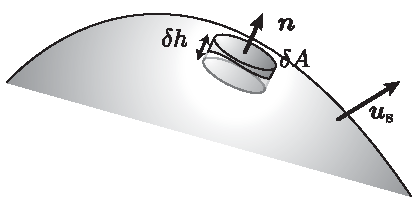
\includegraphics{impermeability.pdf}
\caption{Balance over an elementary volume located across a solid boundary.}
\label{fig:impermeability}
\end{center}
\end{figure}

Let's consider a solid moving in a fluid at velocity $\bu_\text s$ (possibly time dependent) and let's conduct a mass balance on a small cylindrical volume of base $\delA$ and height $\delh$ located across the fluid and the solid (Fig.~\ref{fig:impermeability}). Now let $\delh$ tends to 0 so that the mass element shrinks down to zero.  From now on, the mass variation of the element should necessarily be zero, and this implies that the mass flux from the fluid has to be balanced by the mass flux from the solid side:
\begin{equation}
-\lp\bj_\text{fluid}\cdot \bn_\text{fluid}\rp \delA -  \lp\bj_\text{solid}\cdot \bn_\text{solid}\rp \delA = 0.
\end{equation}
Let's write arbitrarily $\bn = \bn_\text{fluid} = - \bn_\text{solid}$ so that:
\begin{equation}
-\bj_\text{fluid}\cdot \bn +  \bj_\text{solid}\cdot \bn = 0.
\end{equation}
Without mixing phenomena, the fluid velocity $\bu$ already takes into account diffusive effects (it is the chemical species velocity) and the mass flux reduces to the convective flux. Beware that as we are in the solid reference frame, the relative velocity of the fluid is $\bu - \bu_\text s$, so that the mass flux on the fluid side is:
\begin{equation}
\bj_\text{fluid} = \rho \lp\bu-\bu_\text s\rp.
\end{equation}
\prg{The impermeable wall.\index{boundary conditions!impermeability}} A very common case is that of an \textbf{imperméable} solid in which the fluid cannot penetrate; the fluid mass flux within the solid is therefore zero and $\bj_\text{solid} = \boldsymbol 0$. Mass conservation expressed at an impermeable boundary therefore reduces to:
\begin{equation}
\bu\cdot\bn = \bu_\text s \cdot\bn
\label{eq:impermeability}
\end{equation}
This is the \textbf{impermeability condition} for an object (or a wall). As the name implies, it simply expresses the fact that the fluid cannot penetrate into the solid. This condition takes the form of a \textbf{continuity of normal velocities}.

Note: in the quite particular (but still very common!) case of a fixed solid object, this condition reduces to $\bu\cdot\bn =0$.
\prg{Permeable wall.} The previous discussion naturally extends to the case of permeable walls. Those may correspond to biological tissues permeable to given solutes, to materials swollen by solvents, to terrains soaked by rain or to lifting sails or wings made porous in order to control the boundary layer (such as Cousteau and Malavard' turbosail seen in the lecture).

Now the mass flux is non-zero and its precise determination requires a knowledge of the flow \textit{inside} the solid. Suppose however that the imbibition velocity $\bu_\text{imbib}$ be constant and known (this corresponds for example to a suction with an imposed flowrate). The mass conservation at the permeable wall will then be written:
\begin{equation}
\rho (\bu-\bu_\text s) \cdot \bn = \rho (\bu_\text{imbib}) \cdot \bn,
\end{equation}
thus 
\begin{equation}
\bu\cdot\bn = \lp\bu_\text s + \bu_\text{imbib}\rp\cdot\bn.
\end{equation}
\prg{Boundary conditions on a concentration field near a wall.\index{boundary conditions!no-flux}}
The boundary conditions to apply on the transport equation of a concentration field~(\ref{eq:conv_diff}) can be obtainedd following the same principles. Imagine a concentration field transported with a fluid flow $\bu$. Suppose also that an (impermeable) solid is moving in the fluid at velocity $\bu_\text s$. In the solid reference frame the mass flux across any surface $\delA \,\bn$ is:
\begin{equation}
\bj_\text{mass} = \bj_\text{conv} + \bj_\text{diff} = c \lp \bu - \bu_s\rp - D \nabla c.
\end{equation}
The impermeability condition at the wall for the concentration field $c$ is therefore:
\begin{equation}
c (\bu-\bu_\text s) \cdot \bn - D \nabla c \cdot \bn = 0,
\end{equation}
because the mass flux inside the solid is zero.
On using the impermeability condition on the velocity field~(\ref{eq:impermeability}), this relation reduces to:
\begin{equation}
\nabla c \cdot \bn \equiv \pd{c}{n} = 0.
\end{equation}
This Neumann condition is also called a \textbf{no-flux boundary condition.}
\prg{Mass transfer at an interface: evaporation.\index{boundary conditions!evaporation}} One last example of boundary conditions arising from conservation considerations is the continuity of the mass flux across a liquid-gas interface, when the liquid is evaporating.

Let's write a mass balance on a fluid element analogous to the previous one: a small cylindrical element of base $\delA$ and height $\delh$ located across a moving interface with velocity $\bu_\text i$. We let the height $\delh$ of the element tend to zero, so that the element mass equally tends to zero. The mass balance over this element is:
\begin{equation}
\bj_\text{liquid conv.} = \bj_\text{gas conv.} + \bj_\text{gas diff.}
\end{equation}
so that :
\begin{equation}
\rho_\ell \lp\bu_\ell - \bu_\text i\rp \cdot \bn = \rho_v \lp\bu_g -\bu_\text i\rp\cdot \bn - D \nabla \rho_v \cdot n.
\end{equation}
In the case of a violent evaporation (e.g. combustion front), the flux is dominated by convection effects and 
$$\bu_g \sim \underbrace{\frac{\rho_\ell}{\rho_v}}_{\gg 1} \bu_\ell$$
so that the (so-called Stefan) flow induced in the vapour is much stronger than that in the liquid.
In the other limit where evaporation is very slow (case of a slowly drying water drop), it is rather the diffusive term that dominates.
\section{Phenomenological conditions: adherence and continuity}
In addition to the previous boundary conditions arising from conservation principles, fluids are also subject to other boundary conditions as well. The latter have been established and confirmed on experimental grounds, so there is a consensus about their relevance but not an exact demonstration. These phenomenological conditions are \textbf{field continuity conditions} at interfaces and apply on velocity, temperature etc.

\paragraph{$\rhd$ A short history of adherence.\index{boundary conditions!adherence}} The adherence condition $\bu = \bu_\mathrm{s}$ has an astonishing history full of twists and turns, which is accounted for in details in \citet{Goldstein1950}. At the \textsc{xviii}$^\text{th}$ century, the theoretical description of potential flows (corresponding to the idealisation of perfect flow of fluid) was already well established, but the comparisons with experimental data were mediocre. Daniel Bernoulli was well aware of this fact and attributed the discrepancies between (ideal) predicted flows and those observed to some ``adherence condition'' that would prevail at the wall. Coulomb then demonstrated experimentally that an disk oscillating in a liquid was not particularly affected by a change in surface properties (smooth, rough or covered with grease). Therefore it appeared to Coulomb that the fluid velocity matched the disk velocity in its vicinity. In this vision the fluid has the same properties in every point of space; the flow just fulfils an additional condition at the wall.

But during the \textsc{xix}$^\text{th}$ century alternate theories appeared. Girard proposed that the lqiuid layer adjacent to a wall had differing physical properties, leading it to adhere the solid. The next fluid layer (composed of ``regular fluid'') could then freely slip onto the first affixed layer. Navier also got interested into this problem and suggested a boundary condition involving a slip directly proportional to the shear stress $\beta u = \mu \pd{u}{n}$. Here the ratio $\mu/\beta$ has the dimension of a length: it is the \textit{slip length}. From there a period of relative confusion ensued where famous theoreticians of the time (Poisson, Stokes) alternately adopted one or the other of the boundary conditions.

With time however, delicate experiments conducted by Couette or Maxwell advocated definitely for the adherence condition. Maxwell suggested on molecular dynamics considerations that if Navier's condition was effectively valid, the length over which slip occurred was so small -- of the order of a few mean free paths -- that considering it to be zero was a really reasonable hypothesis. This amounted to consider adherence at the wall: $\bu = \bu_\text s$ \citep{Maxwell1879}. This is in particular verified in the usual conditions of laboratory experiments, but not necessarily for rarefied gas flows (e.g. atmospheric reentry, hypersonic flight) or flows involving fluids with long polymer chains (microfluidic flows), as experiments confirm.

During the \textsc{xx}$^\text{th}$ century, the almost perfect agreement between experimental observations and theoretical predictions using adherence condition for a number of flows (Poiseuille flow, Couette flow, Stokes' sphere settlement in a viscous fluid, the instability threshold for the Taylor-Couette experiment etc) definitely settled the validity of this condition.

Moreover, the scaling laws for the drag on an object deduced from dimensional considerations based on the characteristic scales $\rho, U, D$ and $\mu$ capture the evolution of aerodynamic forces over a wide range of scales. If another lengthscale (associated with slip) was relevant in the description of conventional flows, it would result in an alteration of the scaling laws (not observed).

We can understand adherence condition (continuity of $\bu$ across an interface) but also the condition on temperature continuity as resulting from equilibrium at the molecular level. The extremely rapid transfers between neighbouring molecules induce a quasi-instantaneous equilibrium of mean momentum (velocity) and mean thermal agitation velocity (temperature) \citep{Batchelor1967}. At an interface between a medium \textsc{i} and a medium \textsc{ii} (solid-fluid, or fluid-fluid), we will therefore get:
\begin{equation}
\bu_\text{\textsc{i}} = \bu_\text{\textsc{ii}} \quad \text{and} \quad T_\text{\textsc{i}} = T_\text{\textsc{ii}}.
\end{equation}
